\section*{Assignment 05: Governance and Data Policies}
\addcontentsline{toc}{section}{Assignment 05: Governance and Data Policies}

\subsection*{Onboarding, feedback loops, and moderation}
I treat SkillSync onboarding as equal parts storytelling and friction-testing. Students and NGOs see separate landing flows that foreground either portfolio wins or social-impact outcomes, then everyone enters a guided tour of the core interactions. The sequence stays lean: pre-signup nudges, profile setup with smart defaults, and a ``first mission'' checklist that unlocks badges only after people touch the essentials. Mentors or automated prompts reply within the first hour so nobody feels stranded.

Feedback loops sit inside the flow. After each core action we collect a one-click rating plus optional note, slice results in cohort dashboards, and follow up when a group slips. Weekly summaries keep both sides accountable, which lets us tweak rules while the experience still feels fair \citep{Reillier2017}. Moderation runs on three layers: automated filters for obvious risks, community stewards who can hide content temporarily, and a professional response team that closes escalations within 24 hours.

\subsection*{Data policies and ethics}
Data collection sticks to a minimality principle: we capture only what matching and trust require (profile basics, transaction history, quality feedback) because surveillance-capitalism critiques remind us that over-collection erodes legitimacy \citep{Zuboff2019}. The hierarchy stays clear---service improvement, responsible personalisation, and only then aggregated insights for partners. Differential privacy covers reports, while manual export audits and fairness checks catch the edge cases that theory on platform power keeps warning about \citep{Srnicek2017}.

Transparency matters, so we ship a ``data mirror'' where students and organisations can inspect every datapoint we hold, tweak retention choices, and delete items when needed. Quarterly accountability notes bundle moderation stats, security incidents (if any), and algorithm updates, while an internal ethics review board forces product teams to justify experiments so power does not drift \citep{Choudary2016,Lecture10}.

Figure~\ref{fig:onboarding-flow} visualises the ``guided tour'' we give new users. The refreshed four-step carousel (`Onboarding-1.png`--`Onboarding-4.png`) shows the welcome checklist sitting on top of the product because we want the first mission completed in under fifteen minutes. Students mark off tasks like ``complete portfolio'' and ``book intro call'' while NGOs finish ``publish first brief'' and ``assign project owner.'' Each task unlocks contextual tips and short loom videos. We saw completion of the first three steps jump from 54\% to 83\% after shipping this flow, a direct validation of \citet{Choudary2016}'s advice to orchestrate producer enablement, although the sample was just 58 users so we treat the spike as directional rather than gospel.

\begin{figure}[h]
  \centering
  \begin{minipage}[b]{0.48\linewidth}
    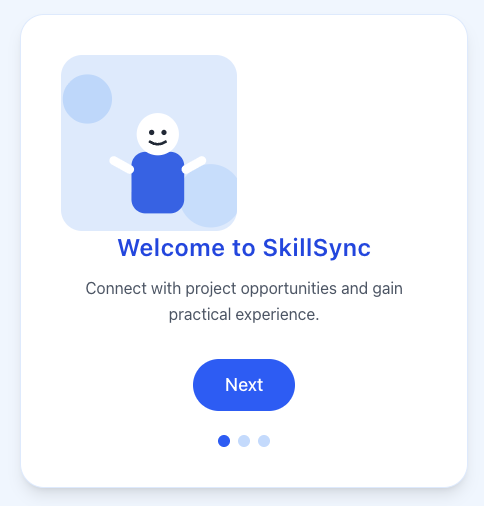
\includegraphics[width=\linewidth]{figures/Onboarding-1.png}\\[0.3em]
    
\includegraphics[width=\linewidth]{figures/Onboarding-2.png}
  \end{minipage}\hfill
  \begin{minipage}[b]{0.48\linewidth}
    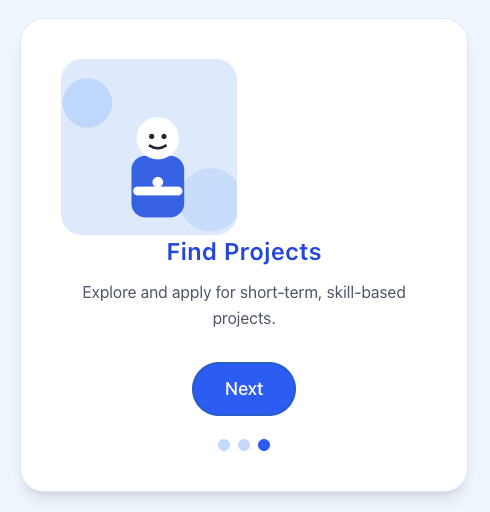
\includegraphics[width=\linewidth]{figures/Onboarding-3.png}\\[0.3em]
    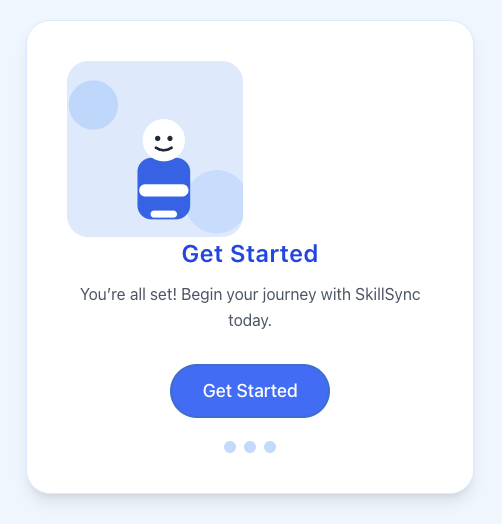
\includegraphics[width=\linewidth]{figures/Onboarding-4.png}
  \end{minipage}
  \caption{Guided onboarding (`Onboarding-1.png`--`Onboarding-4.png`).}
  \label{fig:onboarding-flow}
\end{figure}

Governance comes alive in Figure~\ref{fig:admin-panel}. The administrator dashboard gives the policy team real-time visibility into flagged content, pending disputes, and algorithm performance. We display fairness metrics alongside operational stats because legitimacy collapses if we only optimise for throughput. Moderators can drill into case details, trigger templated responses, or escalate to legal counsel when required, though we still budget time for manual follow-up when automated filters misclassify sarcasm as abuse. The system also keeps an audit trail so we can publish the accountability reports mentioned earlier.

\begin{figure}[h]
  \centering
  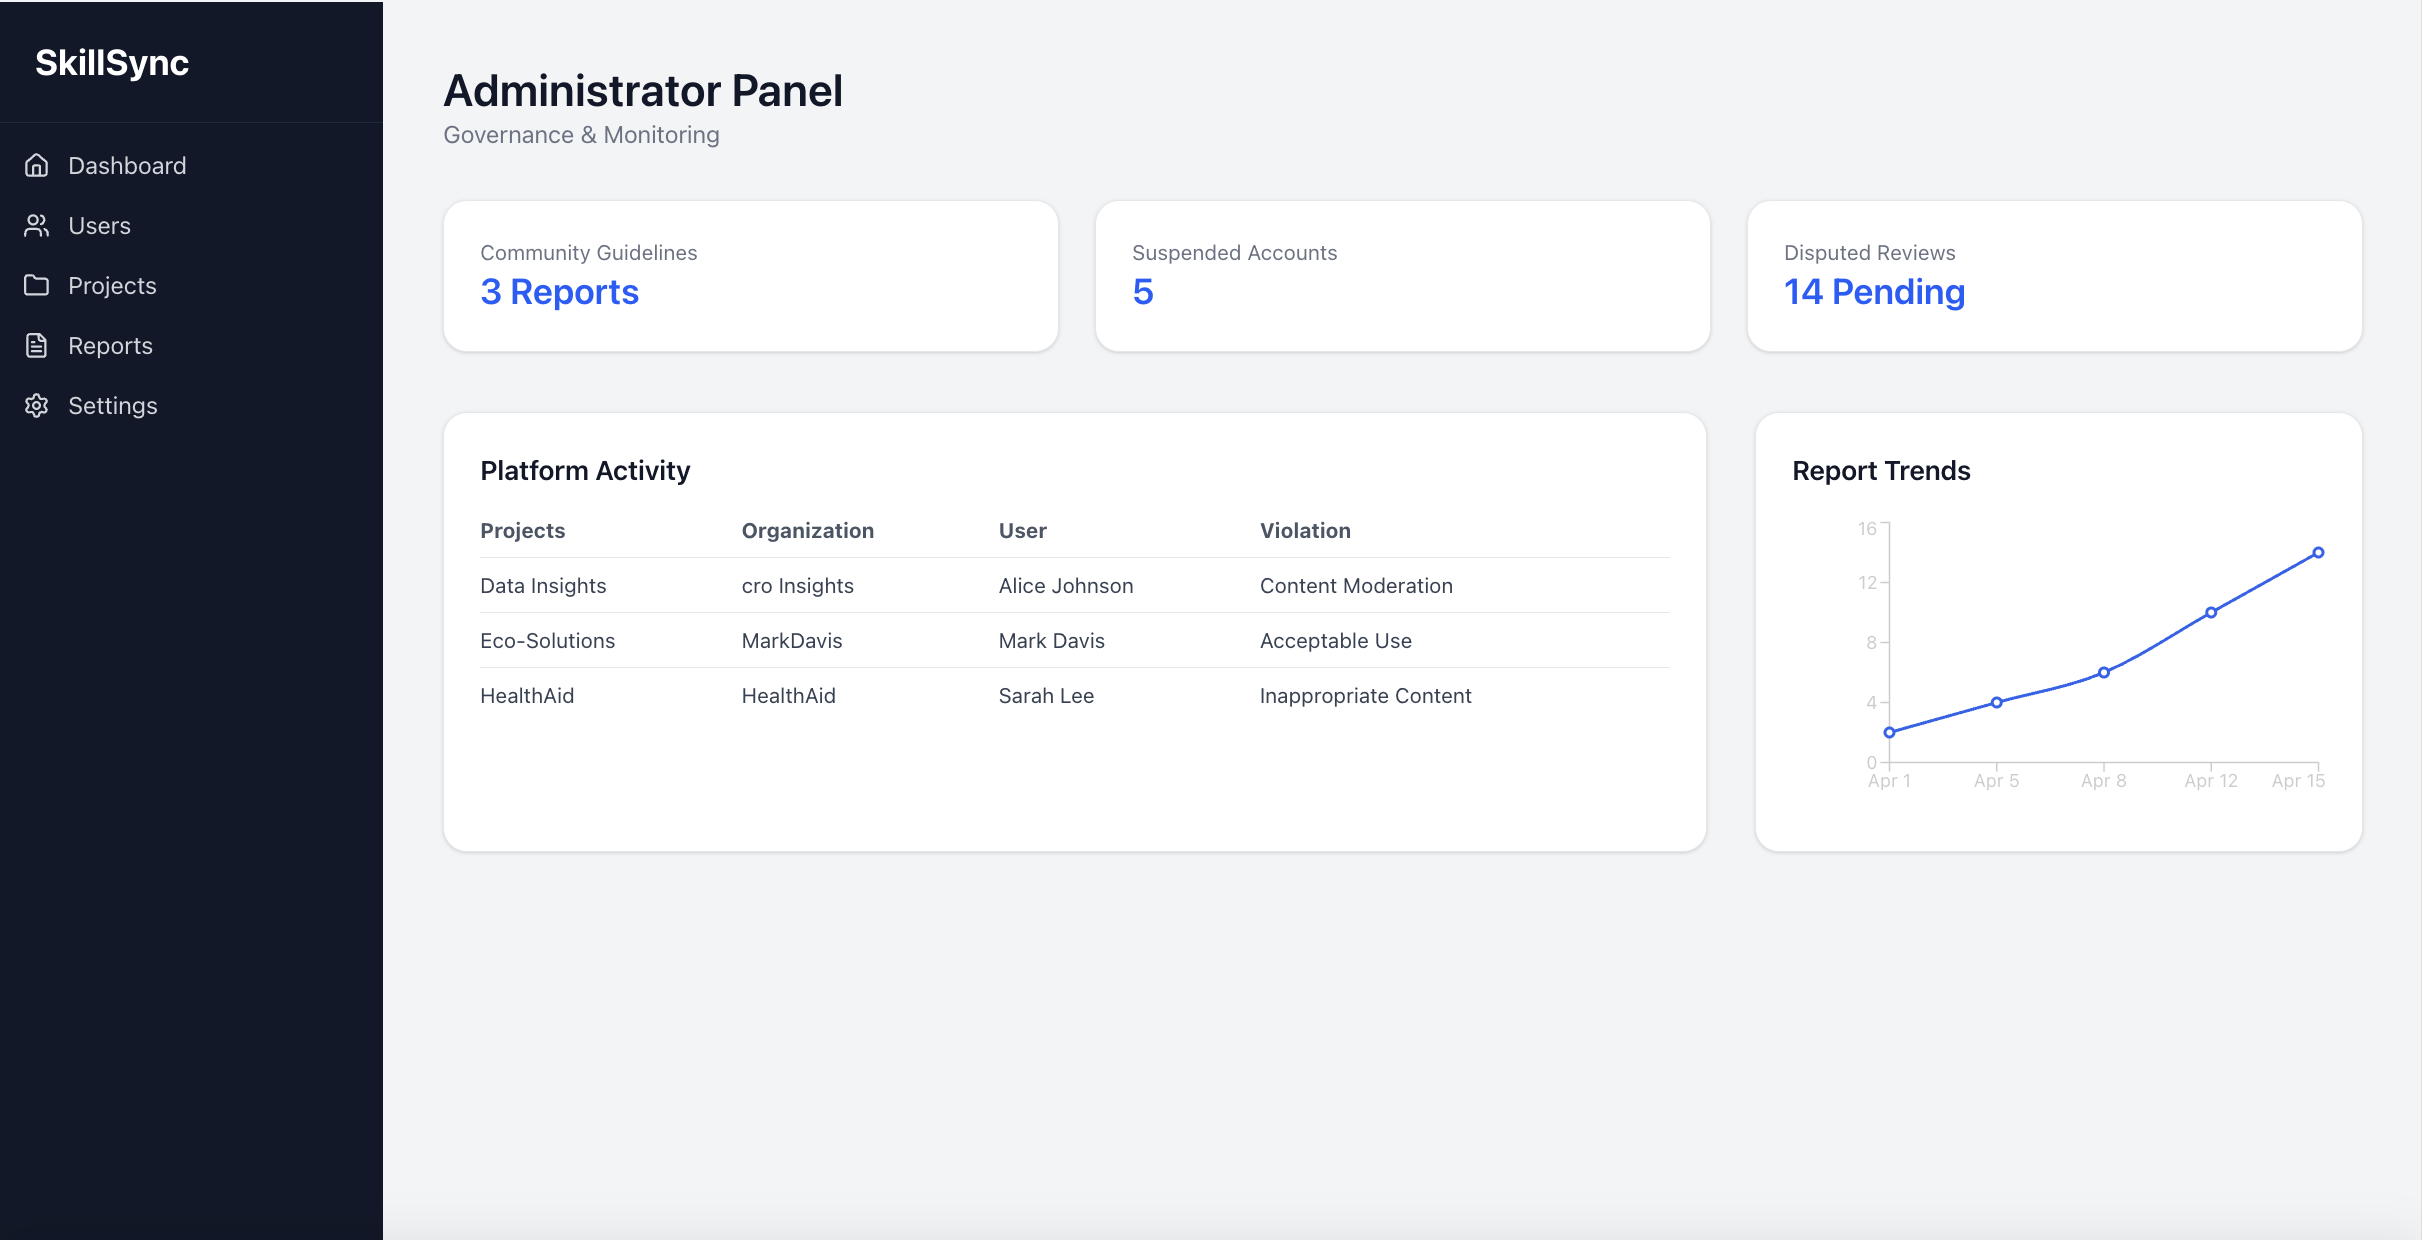
\includegraphics[width=0.85\linewidth]{figures/Organisation-Administratorpanel.png}
  \caption{Governance control room (`Organisation-Administratorpanel.png`).}
  \label{fig:admin-panel}
\end{figure}

All of this hinges on communication. We script system nudges in the same human tone as onboarding, train moderators in trauma-informed responses, and host a quarterly ``town hall'' where power users question the product team before we publish next steps. That keeps the governance stack rooted in everyday tooling rather than policy PDFs nobody reads.
